%\documentclass{opt2026}          % include author names
\documentclass[anon]{opt2026}     % author names withheld for submission

% amsmath, amssymb, natbib, graphicx, url, algorithm2e are loaded by the class.
\usepackage{booktabs}
\usepackage{multirow}
\usepackage{xcolor}

% `proposition' is already provided by the jmlr class loaded by opt2026.
\newcommand{\PH}[1]{\textcolor{red}{\texttt{#1}}}   % placeholder, remove before submission
\newcommand{\PHm}[1]{{\color{red}#1}}                  % placeholder inside math mode
\newcommand{\phirad}{\tilde{\Phi}_{\mathrm{rad}}}
\newcommand{\R}{\mathbb{R}}
\DeclareMathOperator{\Tr}{Tr}

\title[A Soft Constraint Is Not Its Own Limit]{%
  A Soft Constraint Is Not Its Own Limit:\\
  Penalty versus Projection in Sequential SGD}

\optauthor{%
\Name{\PH{Author One}} \Email{\PH{a1@example.edu}}\\
\Name{\PH{Author Two}} \Email{\PH{a2@example.edu}}\\
\addr \PH{Institution}}

\begin{document}
\maketitle

\begin{abstract}%
Penalty and projection methods are two routes to the same constrained solution,
differing in convergence rate rather than in where they arrive. We show that for
a network trained by stochastic gradient descent on a long sequence of tasks,
this equivalence fails. A soft penalty pulling hidden-layer activation norms
toward a fixed radius preserves substantially more of earlier tasks than
unpenalized training, at no cost in current-task accuracy: retention rises from
\PH{20.7}\% to \PH{34.2}\%. Enforcing the same constraint exactly, by projecting
activations onto the sphere, preserves nothing and is marginally worse than no
constraint at all. The two arrive at the same activation geometry and at
different solutions. We derive why. Exact projection makes the layer invariant to
rescaling its weights, so the loss gradient is orthogonal to the weight vector
and the weight norm can only grow: the constraint holds exactly, and the
inflation it was meant to prevent moves into the weights, where nothing opposes
it. The soft penalty leaves the radius in the forward pass and charges for
weight growth. Reducing the step size reproduces the penalty's static geometry
and none of its benefit, and controls that replay its gradient magnitudes
recover none of it either. The effect belongs to the direction of the
optimization path, not to its scale or its endpoint.
\end{abstract}

% =====================================================================
\section{Introduction}
\label{sec:intro}

A constraint can be imposed in two ways: by a penalty that charges for
violating it, with a coefficient $\lambda$ setting the price, or by a projection
that enforces it exactly at every step. In the textbook treatment the two are
interchangeable up to convergence rate: as $\lambda \to \infty$ the penalized
problem approaches the constrained one, and both arrive at the same solution
\citep{nocedal2006numerical}. For a neural network trained by stochastic
gradient descent this need not hold. The two constructions place different
implicit biases on the trajectory, and where the trajectory matters the
solutions can differ even when the constraint is the same. We study a setting in
which the trajectory is all that matters: a network fitted to a long sequence of
tasks, one after another, with no mechanism for remembering earlier ones. How
much of each earlier task survives is a direct readout of how destructive the
optimization path has been.

\paragraph{The constraint.} Let $h \in \R^{d}$ be the pre-activation of a hidden
layer of width $d$. We add to the task loss
\begin{equation}
\label{eq:penalty}
L_{\mathrm{pen}}(h) \;=\; \frac{1}{d}\bigl(\|h\|_2 - \sqrt{d}\bigr)^{2},
\end{equation}
with a single coefficient $\lambda$. This pulls the activation vector toward the
sphere of radius $\sqrt{d}$, which keeps the mean squared activation per unit at
$\mathcal{O}(1)$ and matches standard initialization. Its exact limit is the
projection $h \mapsto \sqrt d\, h / \|h\|_2$, applied in the forward pass. The
same penalty has been studied in the context of delayed generalization on
algorithmic tasks \citep{anon2026radial}; here the question is different.

\paragraph{What we find.} With the soft penalty at small $\lambda$, the network
retains \PH{13.5} points more of earlier tasks than without it, at unchanged
current-task accuracy (\S\ref{sec:observation}). With the constraint enforced
exactly, it retains nothing extra and is slightly worse than the unpenalized
network. The strong penalty and the exact projection end at the same activation
radius, to three digits, and differ by \PH{9.2} points of retention: the
benefit is a property of the path, not of the endpoint. We derive why the exact
limit fails (\S\ref{sec:ratchet}): projection makes the layer scale-invariant in
its weights, so its weight norm is non-decreasing under gradient descent and the
inflation the constraint was meant to stop proceeds in the weights. We show that
the benefit is neither an effective step-size reduction nor a change in gradient
magnitude (\S\ref{sec:controls}), and report what the penalty does change along
the path (\S\ref{sec:path}).

\paragraph{What is new and what is not.} That a scale-invariant layer has
$\langle \nabla_W L, W\rangle = 0$, so that its weight norm grows as
$\|W_{t+1}\|^2 = \|W_t\|^2 + \eta^2\|\nabla_W L\|^2$, is established for
normalization layers \citep{vanlaarhoven2017l2, hoffer2018norm,
arora2019theoretical}, explains how weight decay acts under batch normalization
\citep{zhang2019three}, and motivates optimizers that remove the norm-increasing
component of the update \citep{heo2021adamp}. Our contribution is not the
identity but where it applies: a projection introduced \emph{in order to bound}
activation norms creates exactly the invariance that lets weight norms grow
unopposed, so the constraint defeats its own purpose, and the penalty that only
approximates it does not. Activation-norm penalties are not new
\citep{merity2018regularizing}, and normalization layers impose a hard
per-example version of the same constraint \citep{ba2016layer,
salimans2016weight}; the distinction we care about is soft versus enforced. The
task-sequence setting \citep{goodfellow2013empirical} is an instrument only: we
propose no continual-learning method and do not compare against replay or
parameter-importance schemes \citep{kirkpatrick2017ewc, zenke2017si}, and the
failure mode present is forgetting, not loss of plasticity \citep{dohare2024loss}.

% =====================================================================
\section{Setup}
\label{sec:setup}

\paragraph{Task sequence.} Permuted MNIST: each task applies a fresh fixed
permutation to the input pixels, so every task is equally hard and shares no
input structure with the last. $T = \PH{150}$ tasks, \PH{10} epochs each, no
replay, no task identifier at test time, a single output head. A
\PH{3}-hidden-layer MLP of width $d = \PH{1000}$, ReLU; SGD without momentum at
$\eta = \PH{0.1}$, batch \PH{256}, gradient-norm clip \PH{0.5}; the penalty on
the pre-activations of every hidden layer; \PH{3} seeds per arm unless stated
(Appendix~\ref{app:setup}).

\paragraph{The two ways of imposing the constraint.} The \emph{soft} arms add
$\lambda L_{\mathrm{pen}}$ to the loss at each hidden layer. The \emph{exact}
arm replaces each hidden pre-activation by its projection onto the sphere in the
forward pass, with the projection's true Jacobian in the backward pass; this is
the $\lambda \to \infty$ limit of the soft arm, and amounts to Riemannian
gradient descent on the sphere \citep{absil2008optimization}. We also run
a \emph{straight-through} variant that projects in the forward pass and passes
the gradient through unchanged, a common shortcut that turns out to behave
differently (\S\ref{sec:ratchet}).

\paragraph{Outcome metrics.} \emph{Current-task accuracy} is test accuracy on
the task just fitted. \emph{Retention} is the mean test accuracy over all
previously seen tasks, excluding the current one, measured at each task
boundary. Both are averaged over the final $20$ tasks, where the sequence has
reached a steady state. Definitions in Appendix~\ref{app:metrics}.

\paragraph{Geometric diagnostics.} At each task boundary we record, per layer,
the activation radius $\|h\|_2$ on a fixed probe of \PH{1000} task-$0$ inputs,
the Frobenius norm of the layer's weights, the displacement of the probe
representation since the end of task $0$, and the others listed in
Appendix~\ref{app:metrics}. Nothing is averaged across layers; a quoted
diagnostic is at the first hidden layer unless stated.

% =====================================================================
\section{The observation}
\label{sec:observation}

\begin{table}[!tb]
\centering
\caption{Retention and current-task accuracy against penalty strength, with the
two exactly-enforced arms below the rule. Final $20$ tasks; $n = \PH{3}$ except
$\lambda \in \{0.1, 1\}$ where $n = \PH{2}$. Radius is the first-layer
activation norm on the probe; the sphere target is $\sqrt{1000} = 31.6$. Paired
tests in Appendix~\ref{app:battery}.}
\label{tab:sweep}
\footnotesize
\begin{tabular}{lcccc}
\toprule
Arm & Retention & Current-task acc. & Radius & $\|W\|_F$ \\
\midrule
$\lambda = 0$ (no constraint)  & \PH{0.207} & \PH{0.959} & \PH{49.8} & \PH{50.6} \\
$\lambda = 10^{-4}$            & \PH{0.234} & \PH{0.959} & \PH{49.1} & \PH{50.1} \\
$\lambda = 3\cdot 10^{-3}$     & \textbf{\PH{0.342}} & \PH{0.960} & \PH{43.1} & \PH{45.2} \\
$\lambda = 6\cdot 10^{-3}$     & \PH{0.341} & \PH{0.961} & \PH{40.8} & \PH{43.3} \\
$\lambda = 10^{-2}$            & \PH{0.337} & \PH{0.961} & \PH{38.9} & \PH{41.7} \\
$\lambda = 10^{-1}$            & \PH{0.323} & \PH{0.963} & \PH{31.0} & \PH{33.7} \\
$\lambda = 1$                  & \PH{0.297} & \PH{0.962} & \PH{31.5} & \PH{31.5} \\
$\lambda = 10$                 & \PH{0.291} & \PH{0.962} & \PH{31.6} & \PH{29.8} \\
\midrule
Exact projection               & \PH{0.199} & \PH{0.958} & \PH{31.6} & \PH{48.0} \\
Straight-through projection    & \PH{0.205} & \PH{0.959} & \PH{31.6} & \PH{52.7} \\
\bottomrule
\end{tabular}
\end{table}

Table~\ref{tab:sweep} holds the paper's central measurement.

\paragraph{The soft penalty helps, and the best setting barely enforces the
constraint.} Retention rises from \PH{0.207} to \PH{0.342} at
$\lambda = 3\cdot10^{-3}$, a gain of \PH{0.135} (paired $t = \PH{55.2}$,
$p = \PHm{3\cdot10^{-4}}$, \PH{3/3} seeds), with current-task accuracy unchanged
within \PH{0.2} points. The optimum is a plateau over
$\lambda \in [3\cdot10^{-3}, 6\cdot10^{-3}]$, and there the activation radius is
still \PH{36}\% above the target: the constraint is visibly not satisfied. As
$\lambda$ grows and the radius reaches the sphere, retention declines, but every
soft arm stays well above the baseline.

\paragraph{The exact limit gives nothing.} The exactly projected network pins
the radius to $\sqrt d$ to six digits and retains \PH{0.199}, below the
unconstrained baseline on every seed (paired $t = \PH{-3.4}$, $p = \PH{0.08}$,
\PH{0/3}). The straight-through variant does the same. The entire benefit lives
at finite $\lambda$ and vanishes when the constraint is enforced.

\paragraph{Same endpoint, different solution.} The soft penalty at
$\lambda = 10$ and the exact projection end at the same activation radius,
\PH{31.61} against \PH{31.62}, and differ by \PH{0.092} in retention (paired
$t = \PH{37.9}$, $p = \PHm{7\cdot10^{-4}}$, \PH{3/3}): \PH{68}\% of the whole
effect at the optimum, between two arms whose final activation geometry is
indistinguishable. Whatever the penalty does, it does along the way;
\S\ref{sec:ratchet} derives what the projection does instead.

% =====================================================================
\section{Why the exact limit fails: the weight-norm ratchet}
\label{sec:ratchet}

\begin{proposition}
\label{prop:ratchet}
Let a layer compute $h = Wx$ followed by exact projection
$\Pi(h) = \sqrt{d}\,h/\|h\|_2$. Then $\Pi(Wx)$ is invariant under
$W \mapsto cW$ for every $c > 0$, so the loss is degree-zero homogeneous in
$W$. By Euler's theorem,
\begin{equation}
\label{eq:orthogonal}
\bigl\langle \nabla_W L, \, W \bigr\rangle = 0 ,
\end{equation}
and consequently a gradient step of size $\eta$ satisfies
\begin{equation}
\label{eq:ratchet}
\bigl\| W - \eta \nabla_W L \bigr\|_F^{2}
  \;=\; \|W\|_F^{2} \;+\; \eta^{2}\bigl\|\nabla_W L\bigr\|_F^{2}
  \;\ge\; \|W\|_F^{2}.
\end{equation}
The weight norm is non-decreasing under exact projection, whatever the loss.
Under the soft penalty the corresponding inner product is
\begin{equation}
\label{eq:restoring}
\bigl\langle \nabla_W L_{\mathrm{pen}},\, W \bigr\rangle
  \;=\; \frac{2\lambda}{d}\bigl(\|h\|_2 - \sqrt d\bigr)\|h\|_2 ,
\end{equation}
which is strictly positive whenever $\|h\|_2 > \sqrt d$, so the descent step
reduces $\|W\|_F$. Proofs in Appendix~\ref{app:derivations}.
\end{proposition}

The two constructions differ in exactly the coordinate the constraint is about.
Projection removes the radius from the forward pass, and with it any signal that
the weights have grown; growth is free. The soft penalty leaves the radius in
the forward pass, so growth is visible to the loss and is charged for.
Equation~\eqref{eq:ratchet} is the standard scale-invariance argument
\citep{vanlaarhoven2017l2, arora2019theoretical}; what is new is that here the
invariance is created by a constraint whose stated purpose is to bound the very
quantity it then lets grow.

\paragraph{Prediction.} Under exact projection the activation radius is pinned
and the weight norm inflates across the task sequence anyway. Under the soft
penalty at small $\lambda$, both are arrested.

\paragraph{Result.} Figure~\ref{fig:ratchet} and Table~\ref{tab:ratchet}. Over
$150$ tasks the unconstrained weight norm grows by \PH{+6.0} and its activation
radius by \PH{+4.3}, monotonically. Exact projection holds the radius at
$\sqrt d$ and still grows the weight norm by \PH{+3.3}. The straight-through variant, whose backward
pass is not the Jacobian of a degree-zero map and so does not satisfy
\eqref{eq:orthogonal}, grows it by \PH{+7.6}, more than the baseline. The soft
penalty at $\lambda = 3\cdot10^{-3}$ holds the weight norm to \PH{+0.3} and the
radius to \PH{-1.3}. This explains the same-radius comparison of
\S\ref{sec:observation}: at $\lambda = 10$ the soft arm reaches the sphere with
its weight norm \emph{falling} by \PH{14.3}, while the projected arm reaches the
same sphere with its weight norm rising.

\begin{figure}[!tb]
\centering
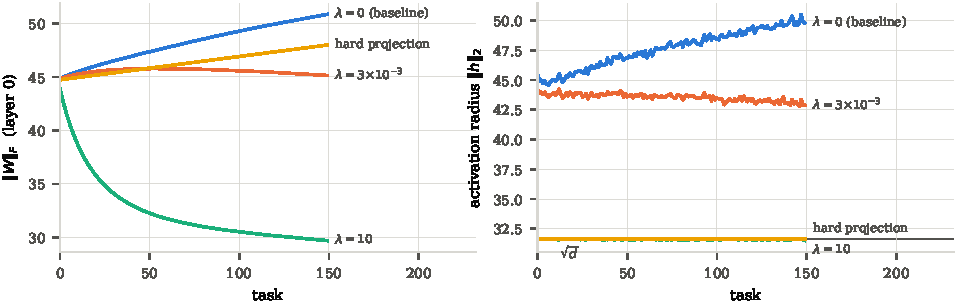
\includegraphics[width=0.72\textwidth]{figs/fig_ratchet.pdf}
\caption{First hidden layer across the task sequence. \textbf{Left}: weight
norm. \textbf{Right}: activation radius on the probe. Exact projection
(``hard projection'' in the legend) pins the radius to $\sqrt d$ and the weight
norm climbs anyway; the soft penalty at $\lambda = 3\cdot10^{-3}$ arrests both.
Two panels rather than one because the two are different measures on different
scales.}
\label{fig:ratchet}
\end{figure}

% =====================================================================
\section{Not the step size, and not the gradient scale}
\label{sec:controls}

Two objections must be answered before the benefit can be attributed to the
direction of the path: that the penalty is an effective step-size reduction,
and that it acts through gradient magnitude alone.

\paragraph{The step size reaches the same geometry and not the same solution.}
Table~\ref{tab:lr}. Lowering $\eta$ from \PH{0.1} to \PH{0.003} without any
penalty reproduces the penalized network's activation radius, weight norm and
effective rank, and reproduces neither its retention nor its accuracy. Across
the step-size sweep, retention falls as $\eta$ rises and accuracy rises with it
($\rho = \PH{-0.77}$, $p = \PH{0.07}$): the step size trades one axis against
the other along a frontier. The penalty sweep lies above that frontier at
\PH{7} of \PH{8} values of $\lambda$, by up to \PH{0.169} in retention at
matched accuracy (Figure~\ref{fig:frontier}, Appendix~\ref{app:battery}).

\begin{table}[!tb]
\centering
\caption{Same geometry, two ways. Reducing the step size reaches the penalty's
radius, weight norm and effective rank at the first hidden layer, and arrives at
a different solution. Full step-size sweep in Appendix~\ref{app:battery}.
Step-size arm $n = \PH{2}$.}
\label{tab:lr}
\small
\begin{tabular}{lcccccc}
\toprule
Arm & Retention & Current-task acc. & Radius & $\|W\|_F$ & Eff.\ rank \\
\midrule
Penalty $\lambda = 3\cdot10^{-3}$, $\eta = 0.1$ & \textbf{\PH{0.342}} & \textbf{\PH{0.960}} & \PH{43.1} & \PH{45.2} & \PH{243.8} \\
No penalty, $\eta = 3\cdot10^{-3}$  & \PH{0.262} & \PH{0.868} & \PH{43.0} & \PH{44.9} & \PH{244.1} \\
\bottomrule
\end{tabular}
\end{table}

\paragraph{Matched gradient magnitudes recover nothing.} Three interventions
replay a recorded scalar from the penalized run onto an unpenalized one, per
seed and per step, carrying no directional information: its gradient magnitude
per parameter group, its total gradient magnitude, and its per-group weight-norm
trajectory. Each must pass a pre-registered matching tolerance before any
outcome is examined, and each is run at a relaxed gradient clip, since the
default clip binds on \PH{89}\% of steps and already pins both arms to the same
total gradient norm (Appendix~\ref{app:controls}). Matching gradient magnitude,
per group or globally, recovers \PH{-1}\% and \PH{-7}\% of the retention gain.
Matching the weight-norm trajectory reproduces the penalized weight norm to
\PH{0.5}\% and recovers \PH{16}\%. A smaller weight norm is a real but minor
part of the story; the remaining \PH{84}\% is not magnitude.

% =====================================================================
\section{What the penalty changes along the path}
\label{sec:path}

The results so far say what the benefit is not. This section reports what the
penalty does change during training. One quantity tracks retention across the
sweep; we present it as a diagnostic, not a mechanism, for reasons given at the
end.

\paragraph{The radial fraction of the task gradient.} The penalty gradient
$\nabla_h L_{\mathrm{pen}} = \tfrac{2}{d}(\|h\|_2 - \sqrt d)\,\hat h$, with
$\hat h = h/\|h\|_2$, points along the activation vector, and in gradient flow
on $h$ the coefficient $\lambda$ enters only the radial coordinate, as a
relaxation time $\tau = d/2\lambda$ of which exact projection is the $\tau = 0$
member (Appendix~\ref{app:flow}). The natural question is therefore what
happens to the task gradient in that direction. With
$P_r = \hat h \hat h^{\top}$ and $g = \nabla_h L_{\mathrm{task}}$ the
\emph{task}-loss gradient only, define
\begin{equation}
\label{eq:phirad}
\phirad \;=\; d \cdot \frac{\|P_r g\|_2^{2}}{\|g\|_2^{2}},
\end{equation}
the share of the task gradient's energy along the activation vector, scaled so
that an isotropic gradient gives $\phirad = 1$. The penalty gradient is excluded
by construction: it is purely radial, and including it would make
\eqref{eq:phirad} a measurement of the regularizer.

\paragraph{It tracks retention at the first hidden layer.} Without the
penalty, the radial share of the first-layer task gradient is \PH{39}\% of its
isotropic value; at $\lambda = 3\cdot10^{-3}$ it is \PH{12}\%
(Table~\ref{tab:phirad}, Appendix~\ref{app:battery}). Across the eight soft
arms $\phirad$ is rank-correlated with retention at $\rho = \PH{-0.905}$,
$p = \PH{0.002}$. The relation is specific to the first hidden layer: at the
second and third layers the correlations are \PH{-0.14} and \PH{-0.17}, neither
significant. The exactly projected arms sit outside the relation entirely. Exact projection deletes the radial component and
reaches $\phirad = 0$, the smallest value possible, with the worst retention of
any arm. A low value of the statistic is therefore not sufficient for the
benefit; it has to be arrived at rather than imposed.

\paragraph{The fall is in the denominator.} Decomposing \eqref{eq:phirad}
between $\lambda = 0$ and $\lambda = 3\cdot10^{-3}$ at the first layer, the
radial component $\|P_r g\|$ changes by \PH{-4.9}\% while the total task
gradient $\|g\|$ changes by \PH{+43.5}\%. The penalty does not suppress the
radial gradient; it enlarges the tangential one, and $\phirad$ falls as a
consequence. The enlargement has a simple account: for cross-entropy with logits
$z = Vh$, $\nabla_h L_{\mathrm{task}} = V^{\top}(\mathrm{softmax}(z) - y)$
vanishes as the correct logit margin grows, so a smaller $\|h\|$ keeps the
softmax away from saturation and leaves a larger task gradient
(Appendix~\ref{app:desat}). This also shows why the diagnostic is not the
mechanism: the exactly projected arm has the largest task gradient of any arm
and the worst retention.

\paragraph{Other diagnostics.} Two other first-layer diagnostics track retention at
the same $\rho = \PH{-0.905}$: the cumulative displacement of the probe
representation since task $0$, and the end-of-task update norm. All three are
close to monotone in $\lambda$, and eight points on a one-dimensional sweep
cannot separate them from one another or from $\lambda$. Radial displacement,
effective and stable rank, subspace overlap and gradient readiness do not track
retention at all (Appendix~\ref{app:battery}). Two negatives constrain the
account: dead units are below $10^{-4}$ in every arm, so the failure mode is
forgetting and not loss of plasticity \citep{dohare2024loss}; and subspace
overlap does not track in any form, which rules out the most natural
representation-preservation explanation.

% =====================================================================
\section{Limitations and conclusion}
\label{sec:conclusion}

Proposition~\ref{prop:ratchet} is the only derived part of the account, and it
explains why the exact limit fails, not why the soft penalty succeeds; the
positive side rests on the same-endpoint comparison and on controls that say
what the benefit is not. The diagnostic of \S\ref{sec:path} is correlational on
eight points and confounded with two other diagnostics and with $\lambda$; the
arm that would separate them, one that lowers $\phirad$ without constraining
the radius, we have not run. This is one task family, one architecture, one
optimizer and \PH{3} seeds (\PH{2} on two sweep points and the step-size
sweep). \PH{TODO:} weight-decay and LayerNorm baselines
(Appendix~\ref{app:aniso}); momentum and Adam; a second task family.

What the evidence supports: a soft activation-norm penalty and its exactly
enforced limit reach the same activation geometry and differ by most of
the effect. The penalty arrests a cumulative inflation of activation and weight
norms; the projection pins the radius, makes the layer scale-invariant in its
weights, and lets the same inflation proceed in weight space unopposed. The
choice between penalty and projection is here a choice of trajectory, not of
convergence rate, and the trajectory is what survives.

\bibliography{refs}

\newpage
\appendix
\section{Metric definitions}
\label{app:metrics}

All quantities are computed at each task boundary and kept per layer. $h$ denotes
pre-activations of the layer in question, $d$ its width.

\paragraph{Accuracy and retention.} Let $a_t^{(k)}$ be accuracy on task $k$'s
held-out set after finishing task $t$, evaluated on the first $\PH{2000}$ test
examples of that task. We report current-task accuracy $a_t^{(t)}$ and retention
$\frac{1}{t}\sum_{k<t} a_t^{(k)}$, which excludes the current task and is
undefined at $t = 0$. We also log
$\frac{1}{t+1}\sum_{k \le t} a_t^{(k)}$, which includes it; the two differ by
$\mathcal{O}(1/t)$ and the second is biased toward arms with higher current-task
accuracy, which is why it is not the reported metric.

\paragraph{Radial quantities.} Radius $\|h\|_2$ and radial excess
$\|h\|_2 - \sqrt d$, both averaged over the probe batch; \texttt{radius\_std} is
the standard deviation of $\|h\|_2$ across probe inputs, which is identically
zero under exact projection.

\paragraph{Radial fraction of the task gradient.} $\phirad$ as in
\eqref{eq:phirad}, with $g$ obtained by \texttt{autograd.grad} of the task loss
with respect to pre-activations. The penalty is never included in the probe
loss. A regression test asserts that passing the total gradient instead changes
the value, and that passing the task gradient reproduces the $\lambda = 0$ value
exactly.

\paragraph{Drift.} On a probe of $\PH{1000}$ task-$0$ inputs, fixed for the run.
For representations $h_{\mathrm{cur}}, h_{\mathrm{ref}}$ we log the absolute
displacement $\|h_{\mathrm{cur}} - h_{\mathrm{ref}}\|_F$, its radial and
tangential parts with respect to $h_{\mathrm{ref}}$, and each divided by
$\|h_{\mathrm{ref}}\|_F$. Two references are used: the previous task boundary
(\emph{consecutive}) and the end of task $0$ (\emph{cumulative}). The relative
forms are reported for comparability with prior work but are not used for
cross-$\lambda$ comparison, since the denominator is a quantity the penalty
directly shrinks.

\paragraph{Subspace overlap.} Top-$k$ left singular subspaces of the two
representation matrices with $k = \PH{50}$ fixed for every arm; overlap is the
mean cosine of the principal angles. Bases are computed in float64 on CPU, which
is deterministic and does not fail on the ill-conditioned matrices that arise at
large $\lambda$.

\paragraph{Rank and units.} Effective rank $\exp(-\sum_i p_i \log p_i)$ with
$p_i = \sigma_i/\sum_j \sigma_j$; stable rank $\|A\|_F^2/\|A\|_2^2$; dead
fraction, the proportion of units with zero output on every probe input; dormant
fraction, the proportion whose mean absolute activation is below $\PH{0.025}$ of
the layer mean.

\paragraph{Readiness.} Over $m = \PH{8}$ microbatches of the probe,
$\|\bar g\|_2 \cdot \|\bar g\|_2^2 / \overline{\|g_i\|_2^2}$, computed
\emph{per layer}.

\section{Derivations}
\label{app:derivations}

\subsection{Proposition~\ref{prop:ratchet}}
$\Pi(cWx) = \sqrt d\,cWx/\|cWx\|_2 = \sqrt d\,Wx/\|Wx\|_2 = \Pi(Wx)$ for $c > 0$,
so the layer's contribution to $L$ satisfies $L(cW) = L(W)$. Differentiating in
$c$ at $c = 1$ gives $\langle \nabla_W L, W\rangle = 0$, which is Euler's theorem
for a degree-zero homogeneous function. Then
\[
\|W - \eta \nabla_W L\|_F^2
 = \|W\|_F^2 - 2\eta\langle \nabla_W L, W\rangle + \eta^2\|\nabla_W L\|_F^2
 = \|W\|_F^2 + \eta^2\|\nabla_W L\|_F^2 ,
\]
which is \eqref{eq:ratchet}. The growth per step is second order in $\eta$ and is
never opposed, so $\|W\|_F$ increases monotonically. This is the mechanism by
which scale-invariant layers accumulate weight norm under normalization
\citep{vanlaarhoven2017l2, arora2019theoretical}; the point here is that it also
applies when the invariance is introduced by a constraint intended to prevent
growth.

For the soft penalty, $\nabla_W L_{\mathrm{pen}} = \frac{2}{d}(r - \sqrt d)\hat h x^\top$
with $r = \|h\|_2$, and $\langle \hat h x^\top, W\rangle = \hat h^\top W x = \hat h^\top h = r$,
giving \eqref{eq:restoring}. Two caveats: the argument is for a single layer with
the projection applied to its own output, and the straight-through variant does
not satisfy \eqref{eq:orthogonal} because its backward pass is not the Jacobian
of a degree-zero map, which is consistent with its inflating faster than the
exact version.

\subsection{Radial--tangential decomposition and the equilibrium law}
\label{app:flow}
With $r = \|h\|_2$ and $\hat h = h/r$,
$\nabla_h L_{\mathrm{pen}} = \frac{2}{d}(r - \sqrt d)\,\hat h$, which lies along
$\hat h$. Writing $u = r - \sqrt d$ and projecting
$\dot h = -\nabla_h L_{\mathrm{total}}$ onto $\hat h$ and its complement gives
\begin{equation}
\label{eq:radial_ode}
\dot u \;=\; -\,g_r \;-\; \frac{2\lambda}{d}\,u ,
\qquad
\dot h_{\mathrm{tan}} \;=\; -(I - P_r)\,\nabla_h L_{\mathrm{task}} .
\end{equation}
The radial equation is linear in $u$ with coefficient $-2\lambda/d$, hence
relaxation time $\tau = d/2\lambda$ and stationary point
$u^\star = -d g_r / 2\lambda$. As $\lambda \to \infty$ the radial mode is
infinitely stiff, $u \to 0$, and only the tangential term survives, which is
gradient flow restricted to $\mathbb{S}^{d-1}(\sqrt d)$.

\paragraph{Prediction.} $\log|u^{\star}|$ against $\log\lambda$ has slope $-1$,
modulo any dependence of $g_r$ on $\lambda$; if $g_r \propto \lambda^{a}$ the
slope is $a-1$.

\paragraph{Result.} Measured log--log slopes of steady-state radial excess are
$\PH{-0.17} \pm \PH{0.16}$ at the first hidden layer and $\PH{-0.93} \pm
\PH{0.31}$ at the second; the third has too few positive-excess points to fit
(Figure~\ref{fig:equilibrium}). The second layer is consistent with both the
naive $-1$ and the corrected $a-1$; the first is consistent with neither. The
idealization is that $h$ is treated as a free variable. In the network $h = Wx$,
so its reachable set is constrained by the parameterization and by a fixed input
distribution, and the descent is on $W$ rather than on $h$. We report the
measured slopes against this caveat rather than claiming the ODE governs the
network.

\begin{figure}[!tb]
\centering
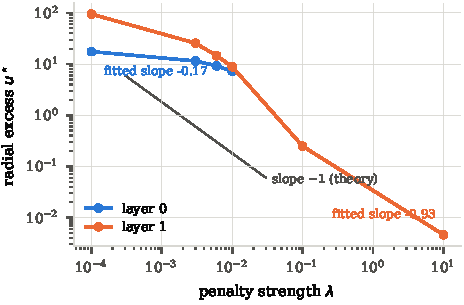
\includegraphics[width=0.6\textwidth]{figs/fig_equilibrium.pdf}
\caption{Steady-state radial excess against $\lambda$, per layer. The second
hidden layer follows the slope $-1$ predicted by \eqref{eq:radial_ode}; the
first is much flatter.}
\label{fig:equilibrium}
\end{figure}

\subsection{Desaturation}
\label{app:desat}
For cross-entropy with logits $z = Vh$,
$\nabla_h L = V^\top(\mathrm{softmax}(z) - y)$. On a correctly classified example
$\mathrm{softmax}(z) \to y$ as the correct logit margin grows, so the residual and
hence $\|\nabla_h L\|$ vanish. Scaling $h$ down scales $z$ down and moves the
softmax away from that regime. The statement is qualitative: it predicts the sign
of the change in $\|\nabla_h L\|$, not its size.

\subsection{The penalty as an anisotropic, task-rotating weight regularizer}
\label{app:aniso}
Under $h = Wx$ and in the inflated regime $\|h\|_2 \gg \sqrt d$, where
$(\|h\|_2-\sqrt d)^2 \approx \|h\|_2^2$,
\begin{equation}
\label{eq:aniso}
\mathbb{E}_x\bigl[L_{\mathrm{pen}}\bigr]
  \;\approx\; \tfrac{1}{d}\,\Tr\!\bigl(W \Sigma_x W^{\top}\bigr),
  \qquad \Sigma_x = \mathbb{E}_x[xx^{\top}] ,
\end{equation}
since $\mathbb{E}_x\|Wx\|_2^2 = \Tr(W\Sigma_x W^\top)$. Unlike
$\lambda\|W\|_F^2$ this weights directions by the variance of the inputs they
read, and in a task sequence $\Sigma_x$ changes with the task, so the axes of
the regularizer rotate with it. The relative error is
$\mathcal{O}(\sqrt d / \|h\|_2)$, which at the unpenalized radius of \PH{49.8}
against $\sqrt d = 31.6$ is roughly \PH{63}\%: the approximation is loose even
where it is best, and we use it only to establish the \emph{form} of the
regularizer. It predicts that an isotropic weight penalty of matched strength
cannot reproduce the benefit, because its axes do not rotate with the task.
\PH{TODO:} weight decay, LayerNorm with weight decay, EWC, SI.

\section{Control construction and acceptance tests}
\label{app:controls}

\begin{table}[!tb]
\centering
\caption{Controls ordered by how much of the penalized signature they reproduce.
Clipping is relaxed here ($\PH{10}$ rather than $\PH{0.5}$) so that a global
magnitude difference exists to be matched; under the default clip both arms are
pinned to the same total gradient norm and the comparison is vacuous.
$n = \PH{3}$. $\phirad$ and radius at the first hidden layer.}
\label{tab:controls}
\small
\begin{tabular}{lcccc}
\toprule
Arm & Retention & $\phirad$ & Radius & $\|W\|_F$ \\
\midrule
Penalty $\lambda = 3\cdot10^{-3}$ & \textbf{\PH{0.305}} & \PH{0.102} & \PH{45.9} & \PH{48.0} \\
Weight-norm matched               & \PH{0.223} & \PH{0.191} & \PH{48.6} & \PH{48.3} \\
Baseline                          & \PH{0.207} & \PH{0.216} & \PH{58.6} & \PH{59.1} \\
Gradient matched, per group       & \PH{0.206} & \PH{0.362} & \PH{58.9} & \PH{59.0} \\
Gradient matched, global          & \PH{0.200} & \PH{0.335} & \PH{57.0} & \PH{57.6} \\
\bottomrule
\end{tabular}
\end{table}

\paragraph{Construction.} Each control arm is trained with $\lambda = 0$ on the
same seed as a completed penalized run, and at every step rescales its own
gradient so that a recorded scalar from the penalized run is reproduced: the
gradient norm per parameter group, the total gradient norm, or, for the
weight-norm arm, the per-group weight norm after the step. The recorded scalars
are read from the penalized run's step-level trace. Any rescaling is applied
\emph{after} gradient clipping; applied before, the clip renormalizes it away and
the intervention silently does nothing (Appendix~\ref{app:setup}).

\paragraph{Acceptance.} Before any outcome is read, each control run must have
a median absolute log-ratio of achieved to target scalar below $0.05$ over all
steps and groups. All three arms pass with a median of \PH{0.00}. Under the default clip
of \PH{0.5} the gradient-matched controls recover \PH{5}\% and \PH{2}\% of the
gain, with the global arm's null uninformative for the reason given in the
caption; the weight-norm arm's acceptance test cannot be run in that regime
because two of its target runs predate the weight-norm trace, and it is
therefore not reported there.

\paragraph{The ordering.} Table~\ref{tab:controls} orders the arms by
retention. The same ordering holds, inverted, for $\phirad$: the only control
that recovers any retention is the only one that lowers $\phirad$, and the two
gradient-magnitude controls raise it above the baseline. The controls were not
designed to test the diagnostic of \S\ref{sec:path}; this is corroboration from
an experiment built for a different purpose.

\section{Full diagnostic tables}
\label{app:battery}

\begin{table}[!tb]
\centering
\caption{Radial fraction of the task gradient per layer, and retention.
$\phirad = 1$ is the isotropic null. Two interpolating rows omitted.}
\label{tab:phirad}
\small
\begin{tabular}{lcccc}
\toprule
Arm & Retention & $\phirad$, layer 1 & layer 2 & layer 3 \\
\midrule
$\lambda = 0$                 & \PH{0.207} & \PH{0.392} & \PH{0.065} & \PH{0.684} \\
$\lambda = 3\cdot 10^{-3}$    & \textbf{\PH{0.342}} & \PH{0.116} & \PH{0.061} & \PH{0.423} \\
$\lambda = 6\cdot 10^{-3}$    & \PH{0.341} & \PH{0.106} & \PH{0.073} & \PH{0.394} \\
$\lambda = 10^{-2}$           & \PH{0.337} & \PH{0.110} & \PH{0.086} & \PH{0.387} \\
$\lambda = 10^{-1}$           & \PH{0.323} & \PH{0.145} & \PH{0.100} & \PH{0.322} \\
$\lambda = 10$                & \PH{0.291} & \PH{0.186} & \PH{0.106} & \PH{0.318} \\
\midrule
Exact projection              & \PH{0.199} & \PH{0.000} & \PH{0.031} & \PH{0.446} \\
Straight-through projection   & \PH{0.205} & \PH{1.035} & \PH{0.197} & \PH{0.574} \\
\bottomrule
\end{tabular}
\end{table}

\begin{table}[!tb]
\centering
\caption{The ratchet, exact values for Figure~\ref{fig:ratchet}. First hidden
layer, first task to last.}
\label{tab:ratchet}
\small
\begin{tabular}{lccc}
\toprule
Arm & $\|W\|_F:\ t_0 \to t_{149}$ & radius$:\ t_0 \to t_{149}$ & Retention \\
\midrule
$\lambda = 0$ (baseline)   & \PH{44.83} $\to$ \PH{50.86} \ (\PH{+6.03}) & \PH{45.47} $\to$ \PH{49.79} \ (\PH{+4.32}) & \PH{0.2067} \\
$\lambda = 3\cdot10^{-3}$  & \PH{44.81} $\to$ \PH{45.14} \ (\textbf{\PH{+0.33}}) & \PH{44.14} $\to$ \PH{42.90} \ (\PH{-1.25}) & \textbf{\PH{0.3416}} \\
$\lambda = 10$             & \PH{43.96} $\to$ \PH{29.69} \ (\PH{-14.27}) & \PH{31.64} $\to$ \PH{31.54} \ (\PH{-0.11}) & \PH{0.2910} \\
Exact projection           & \PH{44.74} $\to$ \PH{47.99} \ (\PH{+3.25}) & \PH{31.62} $\to$ \PH{31.62} \ (\PH{+0.00}) & \PH{0.1994} \\
Straight-through           & \PH{45.10} $\to$ \PH{52.73} \ (\PH{+7.63}) & \PH{31.62} $\to$ \PH{31.62} \ (\PH{+0.00}) & \PH{0.2049} \\
\bottomrule
\end{tabular}
\end{table}

\begin{table}[!tb]
\centering
\caption{Paired comparisons against $\lambda = 0$ on retention, same seeds.
Final $20$ tasks, first hidden layer.}
\label{tab:paired}
\small
\begin{tabular}{lccccc}
\toprule
Arm & $\Delta$ retention & $t$ & $p$ & $n$ & wins \\
\midrule
$\lambda = 10^{-4}$          & \PH{+0.027} & \PH{11.1} & $\PHm{8\cdot10^{-3}}$ & \PH{3} & \PH{3/3} \\
$\lambda = 3\cdot10^{-3}$    & \PH{+0.135} & \PH{55.2} & $\PHm{3\cdot10^{-4}}$ & \PH{3} & \PH{3/3} \\
$\lambda = 6\cdot10^{-3}$    & \PH{+0.134} & \PH{40.4} & $\PHm{6\cdot10^{-4}}$ & \PH{3} & \PH{3/3} \\
$\lambda = 10^{-2}$          & \PH{+0.130} & \PH{29.7} & $\PHm{1\cdot10^{-3}}$ & \PH{3} & \PH{3/3} \\
$\lambda = 10^{-1}$          & \PH{+0.116} & \PH{27.0} & \PH{0.02} & \PH{2} & \PH{2/2} \\
$\lambda = 1$                & \PH{+0.090} & \PH{--} & \PH{--} & \PH{2} & \PH{2/2} \\
$\lambda = 10$               & \PH{+0.084} & \PH{56.4} & $\PHm{3\cdot10^{-4}}$ & \PH{3} & \PH{3/3} \\
Exact projection             & \PH{-0.007} & \PH{-3.4} & \PH{0.08} & \PH{3} & \PH{0/3} \\
Straight-through             & \PH{-0.002} & \PH{-1.4} & \PH{0.30} & \PH{3} & \PH{1/3} \\
\midrule
$\lambda = 10$ vs exact projection & \PH{+0.092} & \PH{37.9} & $\PHm{7\cdot10^{-4}}$ & \PH{3} & \PH{3/3} \\
\bottomrule
\end{tabular}
\end{table}

\begin{figure}[!tb]
\centering
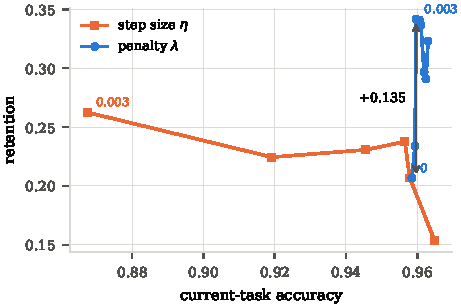
\includegraphics[width=0.6\textwidth]{figs/fig_frontier.pdf}
\caption{The two sweeps in the (current-task accuracy, retention) plane. The step
size traces a trade-off between the axes; the penalty sweep sits above it.}
\label{fig:frontier}
\end{figure}

\begin{table}[!tb]
\centering
\caption{Step-size sweep, no penalty. First hidden layer, final $20$ tasks.
$n = \PH{2}$ except $\eta = 0.3$ where $n = \PH{3}$.}
\label{tab:lrfull}
\small
\begin{tabular}{lcccc}
\toprule
$\eta$ & Retention & Current-task acc. & Radius & $\|W\|_F$ \\
\midrule
$3\cdot10^{-3}$ & \PH{0.262} & \PH{0.868} & \PH{43.0} & \PH{44.9} \\
$10^{-2}$       & \PH{0.225} & \PH{0.919} & \PH{43.6} & \PH{45.1} \\
$2.5\cdot10^{-2}$ & \PH{0.231} & \PH{0.945} & \PH{44.8} & \PH{45.7} \\
$5\cdot10^{-2}$ & \PH{0.238} & \PH{0.957} & \PH{46.7} & \PH{47.2} \\
$10^{-1}$       & \PH{0.207} & \PH{0.958} & \PH{49.8} & \PH{50.6} \\
$3\cdot10^{-1}$ & \PH{0.154} & \PH{0.965} & \PH{67.6} & \PH{68.3} \\
\bottomrule
\end{tabular}
\end{table}

\begin{table}[!tb]
\centering
\caption{Rank correlation with retention across the eight soft arms, first
hidden layer. Quantities that do not track are reported as such.}
\label{tab:battery}
\small
\begin{tabular}{lcc|lcc}
\toprule
Diagnostic & $\rho$ & $p$ & Diagnostic & $\rho$ & $p$ \\
\midrule
$\phirad$                 & \PH{-0.905} & \PH{0.002} & radial drift        & \PH{+0.19} & n.s. \\
cumulative drift from $t_0$ & \PH{-0.905} & \PH{0.002} & effective rank      & \PH{+0.57} & n.s. \\
update norm               & \PH{-0.905} & \PH{0.002} & stable rank         & \PH{+0.57} & n.s. \\
consecutive drift         & \PH{-0.738} & \PH{0.037} & subspace overlap    & \PH{+0.29} & n.s. \\
tangential drift          & \PH{-0.738} & \PH{0.037} & gradient readiness  & \PH{+0.17} & n.s. \\
\bottomrule
\end{tabular}
\end{table}

\PH{TODO:} per-layer columns; the two interpolating $\lambda$ rows of
Table~\ref{tab:phirad}; curvature diagnostics.

\section{Experimental detail and reproducibility}
\label{app:setup}

\paragraph{Configuration.} Permuted MNIST, $\PH{150}$ tasks, one fresh input
permutation per task drawn from the run seed, $\PH{10}$ epochs per task, batch
$\PH{256}$. MLP with $\PH{3}$ hidden layers of width $\PH{1000}$, ReLU, Kaiming
uniform initialization, single $10$-way head shared across tasks, no task
identifier at test time and no replay. SGD without momentum, learning rate
$\PH{0.1}$, global gradient-norm clip $\PH{0.5}$ except where stated. The penalty
is applied to pre-activations of all hidden layers. The exact-projection arm
applies $h \mapsto \sqrt d\, h/\|h\|_2$ to every hidden pre-activation with the
backward pass $(\sqrt d/\|h\|)(I - \hat h \hat h^\top)$; the straight-through
arm applies the same forward map with the identity as backward pass.

\paragraph{Seeds and reporting.} $\PH{3}$ seeds per arm. Every table states $n$.
An arm that has not reached its planned seed count is not reported; comparisons
are paired on seed and give the test statistic, $p$, $n$ and the sign split.
Rank correlations across arms are Spearman.

\paragraph{Gradient clipping and its interaction with the controls.} Under the
default clip of $\PH{0.5}$ the clip binds on $\PH{89}\%$ of steps and pins both
the penalized and unpenalized arms to the same total gradient norm, so the global
magnitude confound is zero by construction and a global-magnitude control has
nothing to remove. The control experiments therefore use a relaxed clip of
$\PH{10}$, which binds on $\PH{46}\%$ of steps and leaves a global magnitude
difference of $\PH{20.1}\%$. Removing clipping entirely is not an option: at
$\eta = \PH{0.1}$ the run diverges, with activation radius reaching $\PH{253}$ by
task $\PH{10}$.

\paragraph{Ordering of gradient operations.} Any rescaling applied to gradients is
applied \emph{after} clipping. Applied before, the clip renormalizes it away and
the intervention silently does nothing. The ordering is asserted at run time and
covered by a regression test.

\paragraph{Numerics.} All spectral quantities are computed on CPU in float64.
The GPU decomposition is not used: it raises on ill-conditioned activation
matrices and its internal fallback is orders of magnitude slower. Any failure
returns NaN and increments a counter that is written into the run's
configuration record, so a run with degraded diagnostics is identifiable.

\paragraph{Records.} Each run writes its complete configuration before training
starts, including every constant that is otherwise implicit (batch size, clip
norm, probe size, method coefficients), a schema version, the code revision, and
the hash of any external input file it consumes. \PH{Code and run records will be
released.}

\end{document}
